\documentclass[10pt]{article}

% Language setting
% Replace `english' with e.g. `spanish' to change the document language
\usepackage[english]{babel}
\usepackage[margin=1cm]{geometry}
% Set page size and margins
% Replace `letterpaper' with `a4paper' for UK/EU standard size
% Useful packages
\usepackage{amsmath}
\usepackage{float}

\usepackage[colorlinks=true, allcolors=blue]{hyperref}
\usepackage{tabularx}
\usepackage{multirow}
\usepackage{mathrsfs}
\usepackage{mathtools}
\usepackage{cite}
\usepackage{amssymb}
\usepackage{caption}
\usepackage{pifont}
\usepackage{verbatim}

\usepackage{textcomp}
\usepackage{tkz-tab}
\usepackage{subcaption}
\usepackage{graphicx}


\begin{document}
\title{Expression of the region of convergence with Gauss-Newton optimization method: Threshold Gaussian With different levels of defocus}
\date{}
\author{Meriem Belinda Naamani}
\maketitle
\section{Expression of the cost function}
\subsection{Expression of the Desired Image}
Assuming a fronto-parallel scene made of a Single 3D bright point at the desired position $\textbf{X}^{*} = \begin{bmatrix}
    X^{*}&Y^{*}&Z^{*}
\end{bmatrix}^{T}\in \mathbb{R}^{3}$ in the camera frame. On a dark textureless background, based on \cite{caron_defocus_based_2021}, the desired image is then given by \eqref{desired_image_eq}.
\begin{equation}
    I_{d}(\textbf{u},\textbf{X}^{*})=\frac{I_{1}}{2\pi\lambda(Z^{*})^{2}} e^{\left(-\frac{||\textbf{u}-pr(\textbf{X}^{*})||^{2}}{2\lambda(Z^{*})^{2}}\right)}
    \label{desired_image_eq}
\end{equation}
Where :
\begin{itemize}
    \item D : aperture diameter
    \item f : focal length
    \item $k_{u}$ : physical size of a pixel
    \item $Z_{f}$ : focus depth
    \item $pr(\textbf{X}^{*})$ is the projection of $\textbf{X}^{*}$ on the circle of confusion and it is given by \eqref{prx}
    \begin{equation}
        pr(\textbf{X}^{*}) = \begin{bmatrix}
    \frac{f}{k_{u}} & 0 & u_{0} \\
    0 & \frac{f}{k_{u}} & v_{0} \\
    0 & 0 & 1
\end{bmatrix}\begin{bmatrix}
    \frac{X^{*}}{Z^{*}}\\
    \frac{Y^{*}}{Z^{*}}\\
    1
\end{bmatrix}
\label{prx}
\end{equation}
\item $\lambda(Z)$ is given by \eqref{lambda}
\begin{equation}
    \lambda (Z) = \frac{Df}{6K_{u}(Z_{f}-f)}\left(1 - \frac{Z_{f}}{Z}\right)
    \label{lambda}
\end{equation}
\end{itemize}

\subsection{Expression of the Current Image}
Applying a translational error on $\textbf{X}^{*}$ the current position is given by $\textbf{X} = \begin{bmatrix}
    X^{*} + tx & Y^{*} + ty & Z^{*} + tz
\end{bmatrix}^{T} \in \mathbb{R}^{3}$. $\textbf{X}$ can be written as $\textbf{X} = \textbf{X}^{*} + \textbf{t}$ where $\textbf{t} = \begin{bmatrix}
    tx & ty & tz
\end{bmatrix}^{T}\in \mathbb{R}^{3}$ The current image is then given by \eqref{current image}.
\begin{equation}
    I_{d}(\textbf{u},\textbf{X})=\frac{I_{1}}{2\pi\lambda(Z^{*}+tz)^{2}} e^{\left(-\frac{||\textbf{u}-pr(\textbf{X})||^{2}}{2\lambda(Z^{*}+tz)^{2}}\right)}
    \label{current image}
\end{equation}

\subsection{Expression of the Cost Function}
Assuming an infinite camera I.e : $\begin{bmatrix} u & v \end{bmatrix} \in \mathbb{R}^{2}$, the cost function can be estimated by \eqref{cost_eq}.
\begin{equation}
    C(\textbf{t}) = \int_{v\in\mathbb{R}}\int_{u\in\mathbb{R}} \frac{1}{2}\left[Id\left(\textbf{u,X}^{*}+\textbf{t}\right) - Id\left(\textbf{u,X}^{*}\right)\right]^{2} du dv
    \label{cost_eq}
\end{equation}
Replacing the current and desired images by \eqref{current image} and \eqref{desired_image_eq}, and using wxmaxima to evaluate the integral the cost function is then given by \eqref{cost_fct_cont}
\begin{equation}
    C(\textbf{t}) = \frac{I_{1}^{2}}{8\pi}\left(\frac{1}{\lambda(Z^{*})^{2}}+\frac{1}{\lambda(Z^{*}+tz)^{2}}\right) -\frac{I_{1}^{2}}{2\pi(\lambda(Z^{*})^{2}+\lambda(Z^{*}+tz)^2)}e^{-\frac{f^{2}\left((X^{*}tz-Z^{*}tx)^{2}+(Y^{*}tz-Z^{*}ty)^{2}\right)}{2(K_{u}Z^{*}(Z^{*}+tz))^{2}(\lambda(Z^{*}+tz)^{2}+\lambda(Z^{*})^{2})}}
    \label{cost_fct_cont}
\end{equation}

\section{Estimation of the region of convergence for optimization with Newton}
\subsection{Estimation of the region of convergence for 2D planar translation}\label{cost_2d_sec}
In this part we consider the controlled degrees of freedom to be 2-D planar translation I.e $\textbf{t} = \begin{bmatrix}
    tx & ty & 0
\end{bmatrix}^{T}$. In that case we have $\lambda(Z^{*}+tz) = \lambda(Z^{*}) = \lambda$. The cost function is then given by \eqref{cost_2D_n}.
\begin{equation}
    C(\textbf{t}) = \frac{I^{2}_{1}}{4\pi\lambda^{2}}\left[1 - exp\left(-\frac{f^{2}(tx^{2}+ty^{2})}{(2K_{u}Z^{*}\lambda)^{2}}\right)\right]
    \label{cost_2D_n}
\end{equation}

The two main conditions to apply the Newton optimization algorithm are given bt \ref{cond}.
\begin{itemize}\label{cond}
    \item \textbf{Condition 1}: the cost function must be twice differentiable.
    \item \textbf{Condition 2}: the hessian matrix needs to be definite positive, I.e : det($\nabla^{2}C(\textbf{t}) \ge 0$)
\end{itemize}
 
The hessian of $C{\textbf{t}}$ is computed using \eqref{hess_eq}.
\begin{equation}
    \nabla^{2} \textbf{C}(\textbf{t}) = \begin{bmatrix}
        \frac{\partial^2C}{\partial tx^{2}}(\textbf{t}) & \frac{\partial^2C}{\partial tx \partial ty}(\textbf{t})\\
        \frac{\partial^2C}{\partial ty \partial tx}(\textbf{t}) & \frac{\partial^2C}{\partial ty^{2}}(\textbf{t})
    \end{bmatrix}
    \label{hess_eq}
\end{equation}
The final expression of the hessian is then given by \eqref{hess}.
\begin{equation}
    \nabla^{2} \textbf{C}(\textbf{t}) = \frac{I^{2}_{1}f^{2}}{8\pi(Z^{*}K_{u}^{2}\lambda^{2})}\\
    \begin{bmatrix}
        1-\frac{f^{2}tx^{2}}{2(Z^{*}K_{u}\lambda)^{2}} & -\frac{f^2txty}{2(Z^{*}K_{u}\lambda)^{2}}\\
        -\frac{f^2txty}{2(Z^{*}K_{u}\lambda)^{2}} & 1-\frac{f^{2}ty^{2}}{2(Z^{*}K_{u}\lambda)^{2}}
    \end{bmatrix}exp\left(-\frac{f^{2}(tx^{2}+ty^{2})}{(2K_{u}Z^{*}\lambda)^{2}}\right)  
    \label{hess}
\end{equation}
In order for the $C{\textbf{t}}$ to be positive definit, then $det(\nabla^{2}C(\textbf{t}))$ given by \eqref{det_H} should be positive.
\begin{equation}
        det(\nabla^{2} \textbf{C}(\textbf{t})) = \frac{I^{2}_{1}f^{2}}{8\pi(Z^{*}K_{u}^{2}\lambda^{2})}\left[\frac{2K_{u}^{2}Z^{*2}\lambda^{2}-f^{2}(tx^2+ty^{2})}{2(K_{u}Z^{*}\lambda)^{2}}\right]exp\left(-\frac{f^{2}(tx^{2}+ty^{2})}{(2K_{u}Z^{*}\lambda)^{2}}\right)
    \label{det_H}
\end{equation}
Solving $det(\nabla^{2}C(\textbf{t}))\geq0$ for $\textbf{t}$,  and replacing $\lambda$ by \eqref{lambda} we obtain \eqref{roc_eq_newton}.
\begin{equation}
    tx^{2}+ty^{2} \leq \frac{D^{2}(Z^{*}-Z_{f})^{2}}{18(Z_{f}-f)^{2}}
    \label{roc_eq_newton}
\end{equation}
The region of convergence is a disk centered at $C = (0.0)$ with a radius of $r_{n} = \frac{\sqrt{2}}{6}D\left(\frac{Z^{2}-Z_{f}}{Z_{f}-f}\right)$.\\Let $r^{2} = tx^{2}+ty^{2}$, the region of convergence is then given by \eqref{roc_newton_polar}
\begin{equation}
    r^{2} \leq \frac{D^{2}(Z^{*}-Z_{f})^{2}}{18(Z_{f}-f)^{2}}
    \label{roc_newton_polar}
\end{equation}
\section{Estimation of the region of convergence for optimization with Gauss-Newton}\label{Gauss_newto_secn}
\subsection{Estimation of the region of convergence for 2D planar translation}
Considering the only controlled DoF are planar translation, as we did in \ref{cost_2d_sec}, the cost function is given by \eqref{cost_2D}.
\par One step of the gauss newton optimization algorithm is given by \eqref{gauss_newton_step}.
\begin{equation}
    \textbf{t}_{k+1} = \textbf{t}_{k} - \left(\left(\frac{\partial \textbf{I}}{\partial \textbf{t}}(\textbf{u},\textbf{t}_{k})\right)^{T}\left(\frac{\partial \textbf{I}}{\partial\textbf{t}}(\textbf{u},\textbf{t}_{k})\right)\right)^{-1}\nabla C(\textbf{t}_{k})
    \label{gauss_newton_step}
\end{equation}
Assuming $\left(\left(\frac{\partial \textbf{I}}{\partial \textbf{t}}(\textbf{u},\textbf{t}_{k})\right)^{T}\left(\frac{\partial \textbf{I}}{\partial\textbf{t}}(\textbf{u},\textbf{t}_{k})\right)\right)$ is not singular. The algorithm stops converging when $\nabla C(\textbf{t}_{k}) = 0$.
When $\nabla C(\textbf{t}_{0}) = 0$, the algorithm either reached the minimum or is stuck in a saddle point surrounding a plateau. \\ The idea is to find these saddle points and plateaux.
\\For the sake of clarity, we omit the \textit{k} subscript in the remainder of this section.
\par The expression of $\nabla C(\textbf{t})$ is given by \eqref{Grad_c}.
\begin{equation}
    \nabla C(\textbf{t}) = \begin{bmatrix}
        \frac{I_{1}^{2}}{4\pi\lambda^{2}}\left(\frac{f^{2}tx}{2(k_{u}Z^{*}\lambda)^{2}}\right)e^{-\frac{f^{2}\left(tx^{2}+ty^{2}\right)}{(2K_{u}Z^{*}\lambda)^{2}}}\\
         \frac{I_{1}^{2}}{4\pi\lambda^{2}}\left(\frac{f^{2}ty}{2(k_{u}Z^{*}\lambda)^{2}}\right)e^{-\frac{f^{2}\left(tx^{2}+ty^{2}\right)}{(2K_{u}Z^{*}\lambda)^{2}}}                 
                    \end{bmatrix}
    \label{Grad_c}
\end{equation}
Solving $\nabla C(\textbf{t}) = 0$ for $\textbf{t}$, the solutions are :

\begin{itemize}
    \item $\textbf{t} = \begin{bmatrix}
        0 & 0 & 0
    \end{bmatrix}^{T}$ 
    \item $\textbf{t} \rightarrow +\infty$
    \item $\textbf{t} \rightarrow -\infty$
\end{itemize}
In this case we conclude that the region of convergence is infinite, and this is due to the fact that the physical limitations of the camera sensor is not taken into considerations. 
\subsection{Bounded Gaussian Model }
Because of the physical limits of the camera sensor, the lowest value capturable value is $\textit{l}\in \mathbb{R}^{*}_{+}$.Thus \eqref{desired_image_eq} can be written as \eqref{desired_image_bounded_1}. 
\begin{equation}
    I_{d}^{*}(\textbf{u}, \textbf{X}^{*})\geq l
    \label{desired_image_bounded_1}
\end{equation}
Replacing $I^{*}_{d}(\textbf{u}, \textbf{X}^{*})$ by \eqref{desired_image_eq}, we obtain \eqref{desired_image_bounded_2}.
\begin{equation}
    \frac{I_{1}}{2\pi\lambda(Z^{*})^{2}} e^{\left(-\frac{||\textbf{u}-pr(\textbf{X}^{*})||^{2}}{2\lambda(Z^{*})^{2}}\right)} \geq l
    \label{desired_image_bounded_2}
\end{equation}
Reorganizing \eqref{desired_image_bounded_2}, we obtain \eqref{desired_image_bounded_3}.
\begin{equation}
    e^{\left(-\frac{||\textbf{u}-pr(\textbf{X}^{*})||^{2}}{2\lambda(Z^{*})^{2}}\right)} \geq \frac{2\pi\lambda(Z^{*})l}{I_{1}}
    \label{desired_image_bounded_3}
\end{equation}
Since the natural logarithm is a monotonic function, applying it on both sides of \eqref{desired_image_bounded_3}, we obtain \eqref{desired_image_bounded_4}
\begin{equation}
    \left(-\frac{||\textbf{u}-pr(\textbf{X}^{*})||^{2}}{2\lambda(Z^{*})^{2}}\right) \geq ln\left(\frac{2\pi\lambda(Z^{*})l}{I_{1}}\right)
    \label{desired_image_bounded_4}
\end{equation}
We then reorganize \eqref{desired_image_bounded_4}, and since we multiply by a negative value, then we direction of the inequality changes obtaining then \eqref{desired_image_bounded_5}.
\begin{equation}
    ||\textbf{u}-\textbf{X}^{*}||^{2} \leq -2\lambda(Z^{*})^{2} ln\left(\frac{2\pi\lambda(Z^{*})l}{I_{1}}\right)
    \label{desired_image_bounded_5}
\end{equation}
Finally, the desired image expression is given by \eqref{desired_image_bounded}
\begin{equation}
    I_{d}^{*}(\textbf{u}, \textbf{X}^{*})
    \begin{cases}
        \frac{I_{1}}{2\pi\lambda(Z^{*})^{2}} e^{\left(-\frac{||\textbf{u}-pr(\textbf{X}^{*})||^{2}}{2\lambda(Z^{*})^{2}}\right)} & \text{if } ||\textbf{u}-\textbf{X}^{*}||^{2} \leq -2\lambda(Z^{*})^{2} ln\left(\frac{2\pi\lambda(Z^{*})l}{I_{1}}\right)\\
        l & \text{Otherwise}
    \end{cases}
    \label{desired_image_bounded}
\end{equation}
Following the same steps we can deduce the expression of the curent image $I_{d}(\textbf{u}, \textbf{X})$, and it is given by \eqref{current_image_bounded}
\begin{equation}
    I_{d}^{*}(\textbf{u}, \textbf{X})
    \begin{cases}
        \frac{I_{1}}{2\pi\lambda(Z^{*}+tz)^{2}} e^{\left(-\frac{||\textbf{u}-pr(\textbf{X})||^{2}}{2\lambda(Z^{*}+tz)^{2}}\right)} & \text{if } ||\textbf{u}-\textbf{X}||^{2} \leq -2\lambda(Z^{*}+tz)^{2} ln\left(\frac{2\pi\lambda(Z^{*}+tz)l}{I_{1}}\right)\\
        l & \text{Otherwise}
    \end{cases}
    \label{current_image_bounded}
\end{equation}
\subsection{Estimation of the cost Function}
The current and desired images are piecewise functions, in that case, we can destinguish two cases for the integral : \textbf{Overlap between the Gaussians} and \textbf{No overlap between the Gaussians}
\subsubsection{No overlap between the current and desired Gaussians}\label{no_overlap_section}
In this case we consider that there is no overlap between the gaussian parts of the two images, as shown in figure \ref{no_overlap}. \\
\begin{figure}[h!]
        \centering
        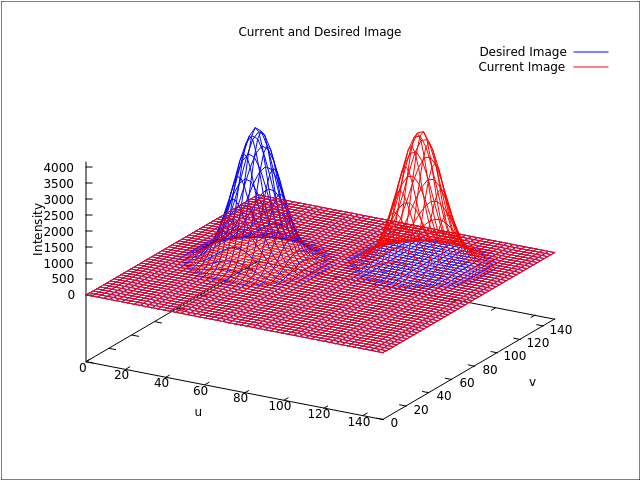
\includegraphics[scale = 0.5]{figures/no_overlap.png}
        \caption{Current amd desired image }
        \label{no_overlap}
\end{figure}
The range of definition of the gaussian portion of the desired image is a disk centered at "$o_{1} = pr(\textbf{X}^{*})$" with a radius of \\ $r_{d}=\sqrt{-2\lambda(Z^{*})^{2} ln\left( \frac{2\pi\lambda(Z^{*})^{2}}{I_{1}}\right)} $
, and at "$o_{2}$=pr($\textbf{X}^{*}$+\textbf{t})" with a radius of $r = \sqrt{-2\lambda(Z^{*}+tz)^{2} ln\left( \frac{2\pi\lambda(Z^{*}+tz)^{2}}{I_{1}}\right)}$ for the current image. We consider that there is 
an overlap if the distance between the two centers of the definition domain of the two gaussian is larger than then sum of the two radii I.e : d($o_{1},o_{2}) \geq r +r_{d}$ . Mathematically is can be written as \eqref{no_over_cond}
\begin{equation} \label{no_over_cond}
    \begin{split}
        \resizebox{0.9\hsize}{!}{$||pr(\textbf{X}^{*}+\textbf{t})-pr(\textbf{X}^{*})|| \geq \sqrt{-2\lambda(Z^{*}+tz)^{2} ln\left( \frac{2\pi\lambda(Z^{*}+tz)^{2}}{I_{1}}\right)}+ \sqrt{-2\lambda(Z^{*})^{2} ln\left( \frac{2\pi\lambda(Z^{*})^{2}}{I_{1}}\right)}$}\\
        \resizebox{0.9\hsize}{!}{$\frac{f}{K_{u}Z\left(tz+Z\right)}\sqrt{\left(Xtz-Z^{*}tx\right)^{2}+\left(Ytz-Z^{*}ty\right)^{2}} \geq \sqrt{-2\lambda(Z^{*}+tz)^{2} ln\left( \frac{2\pi\lambda(Z^{*}+tz)^{2}}{I_{1}}\right)}+ \sqrt{-2\lambda(Z^{*})^{2} ln\left( \frac{2\pi\lambda(Z^{*})^{2}}{I_{1}}\right)} $}\\
        \resizebox{0.9\hsize}{!}{$\sqrt{\left(Xtz-Z^{*}tx\right)^{2}+\left(Ytz-Z^{*}ty\right)^{2}} \geq \frac{K_{u}Z\left(tz+Z^{*}\right)}{f} \left(\sqrt{-2\lambda(Z^{*}+tz)^{2} ln\left( \frac{2\pi\lambda(Z^{*}+tz)^{2}}{I_{1}}\right)}+ \sqrt{-2\lambda(Z^{*})^{2} ln\left( \frac{2\pi\lambda(Z^{*})^{2}}{I_{1}}\right)} \right)$}
    \end{split}  
\end{equation}
So \eqref{cost_eq} in the case of no overlap becomes \eqref{cost_eq_1}
\begin{equation}
    C(\textbf{t})= \int_{v\in\mathbb{V}}\int_{u\in\mathbb{U}} \frac{1}{2}Id\left(\textbf{u,X}\right)^{2} + \frac{1}{2}Id\left(\textbf{u,X}^{*}\right)^{2} du dv
\label{cost_eq_1}
\end{equation} 
To simplify the computations, we convert to the polar coordinates, for the desired image we set \\r1 = $||\textbf{u}-pr(\textbf{X}^{*})||$, and r2 = $ ||\textbf{u}-pr(\textbf{X})||$ for the current image. So the expression of the integral is given by \eqref{cost_eq_2} 
\begin{equation}
    C(\textbf{t}) = \frac{1}{2}\left(\int_{0}^{2\pi}\int_{0}^{\sqrt{-2\lambda(Z^{*})^{2} ln\left( \frac{2\pi\lambda(Z^{*})^{2}}{I_{1}}\right)}} r_{1} e^{\frac{-r_{1}^{2}}{\lambda(Z^{*})^{2}}} dr_{1}d\theta + \int_{0}^{2\pi}\int_{0}^{\sqrt{-2\lambda(Z^{*}+tz)^{2} ln\left( \frac{2\pi\lambda(Z^{*}+tz)^{2}}{I_{1}}\right)}} r_{2} e^{\frac{-r_{2}^{2}}{\lambda(Z^{*}+tz)^{2}}} dr_{2}d\theta \right)
    \label{cost_eq_2}
\end{equation}
Using WxMaxima to estimate the integral, we find the expression in \eqref{cost_eq_3}
\begin{equation}
C(\textbf{t}) = \frac{1}{2}\left[\frac{I_{1}^{2}}{4\pi\lambda(Z^{*}+tz)^{2}}\left(1-\frac{4l\pi\lambda(Z^{*}+tz)^{2}}{I_{1}}e^{\left(-4\lambda(tz+Z^{*})^{2}\right)}\right)+\frac{I_{1}^{2}}{4\pi\lambda(Z^{*})^{2}}\left(1-\frac{4l\pi\lambda(Z^{*})^{2}}{I_{1}}e^{\left(-4\lambda(Z^{*})^{2}\right)}\right)\right]
\label{cost_eq_3}
\end{equation}
Considering that $l\rightarrow 0$, we obtain the result in expression \eqref{cost_no_overlap}.
\begin{equation}
C(\textbf{t}) =  \frac{I_{1}^{2}}{8\pi}\left(\frac{1}{\lambda(Z^{*})^{2}}+\frac{1}{\lambda(Z^{*}+tz)^{2}}\right)
\label{cost_no_overlap}
\end{equation}

\subsubsection{Overlap between the current and desired Gaussians}\label{overlap_section}
In this case we consider the overlap between the two gaussian parts of the image the range of definition as shown in figure \ref{overlap}. 
\begin{figure}[h!]
    \centering
    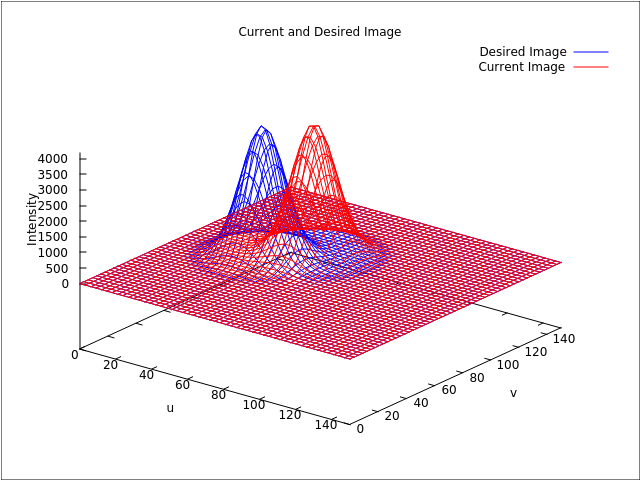
\includegraphics[scale = 0.5]{figures/overlap.png}
    \caption{Current amd desired image }
    \label{overlap}
\end{figure}
Following the same process as in section \ref{no_overlap_section}, the region where the two gaussians overlaps, is given \eqref{overlap_range}.
\begin{equation}
    \resizebox{.9\hsize}{!}{$\sqrt{\left(Xtz-Z^{*}tx\right)^{2}+\left(Ytz-Z^{*}ty\right)^{2}} < \frac{K_{u}Z^{*}\left(tz+Z\right)}{f} \left(\sqrt{-2\lambda(Z^{*}+tz)^{2} ln\left( \frac{2\pi\lambda(Z^{*}+tz)^{2}l}{I_{1}}\right)}+ \sqrt{-2\lambda(Z^{*})^{2} ln\left( \frac{2\pi\lambda(Z^{*})^{2}l}{I_{1}}\right)} \right)$}
    \label{overlap_range}
\end{equation}

The region of integration is given by the region of intersection between the two disks of equations \eqref{current_disk} and \eqref{desired_disk} for the current and desired image respectively
\begin{subequations}
    \begin{equation}
        ||\textbf{u}-pr(\textbf{X}^{*}+\textbf{t})||^{2} = -2\lambda(Z^{*}+tz)^{2} ln\left( \frac{2\pi\lambda(Z^{*}+tz)^{2}l}{I_{1}}\right)
        \label{current_disk}
    \end{equation}
    \begin{equation}
        ||\textbf{u}-pr(\textbf{X}^{*})||^{2} = -2\lambda(Z^{*})^{2} ln\left( \frac{2\pi\lambda(Z^{*})^{2}l}{I_{1}}\right)
        \label{desired_disk}
    \end{equation}
    \label{disks equation}
\end{subequations}
Replacing $pr(\textbf{X}^{*})$ and $pr(\textbf{X}^{*}+\textbf{t})$ with their expression we obtain \eqref{disk1} and \eqref{disk2}.
\begin{subequations}
    \begin{equation}
        \resizebox{.9\hsize}{!}{$\left(u - \frac{f}{K_{u}(Z^{*}+tz)}(X^{*}+tx) - u_{0}\right)^{2}+ \left(v - \frac{f}{K_{u}(Z^{*}+tz)}(Y^{*}+ty) - v_{0}\right)^{2} = -2\lambda(Z^{*}+tz)^{2} ln\left( \frac{2\pi\lambda(Z^{*}+tz)^{2}l}{I_{1}}\right)$}
        \label{disk1}
    \end{equation}
    \begin{equation}
        \resizebox{0.8\hsize}{!}{$\left(u - \frac{f}{K_{u}(Z^{*})}(X^{*}) - u_{0}\right)^{2}+ \left(v - \frac{f}{K_{u}(Z^{*})}(Y^{*}) - v_{0}\right)^{2} = -2\lambda(Z^{*})^{2} ln\left( \frac{2\pi\lambda(Z^{*})^{2}l}{I_{1}}\right)$}
        \label{disk2}
    \end{equation}
\end{subequations}
From \eqref{disk2} we have \eqref{u1} and \eqref{u2}.
\begin{subequations}
    \begin{equation}
        \resizebox{.9\hsize}{!}{$u_{1} = \frac{f}{K_{u}(Z^{*}+tz)}(X^{*}+tx) + u_{0} - \sqrt{-2\lambda(Z^{*})^{2} ln\left( \frac{2\pi\lambda(Z^{*})^{2}l}{I_{1}}\right) -\left(v - \frac{f}{K_{u}(Z^{*})}(Y^{*}) - v_{0}\right)^{2}}$}
        \label{u1}
    \end{equation}
    \begin{equation}
        \resizebox{.9\hsize}{!}{$u_{2} = \frac{f}{K_{u}(Z^{*}+tz)}(X^{*}+tx) + u_{0} + \sqrt{-2\lambda(Z^{*})^{2} ln\left( \frac{2\pi\lambda(Z^{*})^{2}l}{I_{1}}\right) -\left(v - \frac{f}{K_{u}(Z^{*})}(Y^{*}) - v_{0}\right)^{2}}$}
        \label{u2}
    \end{equation}
\end{subequations}
Replacing with \eqref{u1} and \eqref{u2} in \eqref{disk1} and solving for v, we obtain \eqref{v1} and \eqref{v2}.
\begin{subequations}
    \begin{equation}
        v1 = \alpha +\mathit{v0}+\frac{f\, \left( \mathit{ty}+Y^{*}\right) }{\mathit{K_{u}}\, \left( \mathit{tz}+Z^{*}\right) }-\beta
        \label{v1}
    \end{equation}
    \begin{equation}
        v2 = \alpha +\mathit{v0}+\frac{f\, \left( \mathit{ty}+Y^{*}\right) }{\mathit{K_{u}}\, \left( \mathit{tz}+Z^{*}\right) }+\beta
        \label{v2}
    \end{equation}
\end{subequations}
with :
\begin{itemize}
    \item $\alpha = \frac{\left( \frac{Y^{*} f}{\mathit{K_{u}} Z^{*}}-\frac{f\, \left( \mathit{ty}+Y^{*}\right) }{\mathit{K_{u}}\, \left( \mathit{tz}+Z^{*}\right) }\right) \, \left( -4 {{{\lambda }(Z^{*})}^{4}} {{\ln{\left( \frac{2 {l_1} pi {{{\lambda }(Z^{*})}^{2}}}{\mathit{I1}}\right) }}^{2}}+4 {{\lambda }(Z^{*}+tz)^{4}}\, {{\ln{\left( \frac{2 {l_1} pi {{\lambda }(Z^{*}+tz)^{2}}}{\mathit{I1}}\right) }}^{2}}+{{\left(\frac{Y^{*} f}{\mathit{K_{u}} Z^{*}}-\frac{f\, \left( \mathit{tx}+Y\right) }{\mathit{K_{u}}\, \left( \mathit{tz}+Z^{*}\right) }\right) }^{2}}+{{\left( \frac{X^{*} f}{\mathit{K_{u}} Z}-\frac{f\, \left( \mathit{tx}+X^{*}\right) }{\mathit{K_{u}}\, \left( \mathit{tz}+Z^{*}\right) }\right) }^{2}}\right) }{2 \left( {{\left( \frac{Y^{*} f}{\mathit{K_{u}} Z}-\frac{f\, \left( \mathit{tx}+Y\right) }{\mathit{K_{u}}\, \left( \mathit{tz}+Z^{*}\right) }\right) }^{2}}+{{\left( \frac{X^{*} f}{\mathit{K_{u}} Z}-\frac{f\, \left( \mathit{tx}+X^{*}\right) }{\mathit{K_{u}}\, \left( \mathit{tz}+Z^{*}\right) }\right) }^{2}}\right) }$
    \item $\beta = \frac{\left( \frac{f\, \left( \mathit{tx}+X^{*}\right) }{\mathit{K_{u}}\, \left( \mathit{tz}+Z\right) }-\frac{X^{*} f}{\mathit{K_{u}} Z}\right) \, \sqrt{4 {{\lambda }^{4}}\, {{\ln{\left( \frac{2 {l_1} pi {{\lambda }^{2}}}{\mathit{I1}}\right) }}^{2}}-\frac{{{\left( -4 {{{{\lambda }_d}}^{4}} {{\ln{\left( \frac{2 {l_1} pi {{{{\lambda }_d}}^{2}}}{\mathit{I1}}\right) }}^{2}}+4 {{\lambda }^{4}}\, {{\ln{\left( \frac{2 {l_1} pi {{\lambda }^{2}}}{\mathit{I1}}\right) }}^{2}}+{{\left( \frac{Y^{*} f}{\mathit{K_{u}} Z}-\frac{f\, \left( \mathit{tx}+Y\right) }{\mathit{K_{u}}\, \left( \mathit{tz}+Z\right) }\right) }^{2}}+{{\left( \frac{X^{*} f}{\mathit{K_{u}} Z}-\frac{f\, \left( \mathit{tx}+X^{*}\right) }{\mathit{K_{u}}\, \left( \mathit{tz}+Z\right) }\right) }^{2}}\right) }^{2}}}{4 \left( {{\left( \frac{Y^{*} f}{\mathit{K_{u}} Z}-\frac{f\, \left( \mathit{tx}+Y\right) }{\mathit{K_{u}}\, \left( \mathit{tz}+Z\right) }\right) }^{2}}+{{\left( \frac{X^{*} f}{\mathit{K_{u}} Z}-\frac{f\, \left( \mathit{tx}+X^{*}\right) }{\mathit{K_{u}}\, \left( \mathit{tz}+Z\right) }\right) }^{2}}\right) }}}{\sqrt{{{\left( \frac{Y^{*} f}{\mathit{K_{u}} Z}-\frac{f\, \left( \mathit{tx}+Y\right) }{\mathit{K_{u}}\, \left( \mathit{tz}+Z\right) }\right) }^{2}}+{{\left( \frac{X^{*} f}{\mathit{K_{u}} Z}-\frac{f\, \left( \mathit{tx}+X^{*}\right) }{\mathit{K_{u}}\, \left( \mathit{tz}+Z\right) }\right) }^{2}}}} $
\end{itemize}
Now \eqref{cost_eq} becomes :
\begin{equation}
    \resizebox{.9\hsize}{!}{$C(\textbf{t})=\frac{1}{2}\left(\int_{0}^{2\pi}\int_{0}^{\sqrt{-2\lambda(Z^{*})^{2} ln\left( \frac{2\pi\lambda(Z^{*})^{2}}{I_{1}}\right)}} r_{1} e^{\frac{-r_{1}^{2}}{\lambda(Z^{*})^{2}}} dr_{1}d\theta + \int_{0}^{2\pi}\int_{0}^{\sqrt{-2\lambda(Z^{*}+tz)^{2} ln\left( \frac{2\pi\lambda(Z^{*}+tz)^{2}}{I_{1}}\right)}} r_{2} e^{\frac{-r_{2}^{2}}{\lambda(Z^{*}+tz)^{2}}} dr_{2}d\theta \right) - \int_{v1}^{v2}\int_{u1}^{u2}  \frac{I_{1}}{2\pi\lambda(Z^{*}+tz)^{2}} e^{\left(-\frac{||\textbf{u}-pr(\textbf{X}^{*}+\textbf{t})||^{2}}{2\lambda(Z^{*}+tz)^{2}}\right)} \frac{I_{1}}{2\pi\lambda(Z^{*})^{2}} e^{\left(-\frac{||\textbf{u}-pr(\textbf{X}^{*})||^{2}}{2\lambda(Z^{*})^{2}}\right)}  du dv$}
    \label{int_u1,v1}
\end{equation}
We integrate using WxMaxima, and with $l\rightarrow 0$, the cost function is given by \eqref{cost_eq_overlap}.
\begin{equation}
    C(\textbf{t})=\frac{I_{1}^{2}}{8\pi}\left(\frac{1}{\lambda(Z^{*})^{2}}+\frac{1}{\lambda(Z^{*}+tz)^{2}}\right) -\frac{I_{1}^{2}}{2\pi(\lambda(Z^{*})^{2}+\lambda(Z^{*}+tz)^2)}e^{-\frac{\left(\frac{f}{K_{u}Z(Z+tz)}\right)^{2}\left((Xtz-Ztx)^{2}+(Ytz-Zty)^{2}\right)}{2(\lambda(Z+tz)^{2}+\lambda(Z)^{2})}}
    \label{cost_eq_overlap}
\end{equation}
\subsubsection{Final Cost Function}
Considering the results in \ref{no_overlap_section} and \ref{overlap_section} the cost function is then given by \eqref{final_cost_function}.
\begin{equation}
    C(\textbf{t}) = 
    \begin{cases}
        \frac{I_{1}^{2}}{8\pi}\left(\frac{1}{\lambda(Z^{*})^{2}}+\frac{1}{\lambda(Z^{*}+tz)^{2}}\right) \text{if } \resizebox{.7\hsize}{!}{$\sqrt{\left(Xtz-Z^{*}tx\right)^{2}+\left(Ytz-Z^{*}ty\right)^{2}} \geq \frac{K_{u}Z^{*}\left(tz+Z^{*}\right)}{f} \left(\sqrt{-2\lambda(Z^{*}+tz)^{2} ln\left( \frac{2\pi\lambda(Z^{*}+tz)^{2}l}{I_{1}}\right)}+ \sqrt{-2\lambda(Z^{*})^{2} ln\left( \frac{2\pi\lambda(Z^{*})^{2}l}{I_{1}}\right)} \right)$} & \\
        \frac{I_{1}^{2}}{8\pi}\left(\frac{1}{\lambda(Z^{*})^{2}}+\frac{1}{\lambda(Z^{*}+tz)^{2}}\right) -\frac{I_{1}^{2}}{2\pi(\lambda(Z^{*})^{2}+\lambda(Z^{*}+tz)^2)}e^{-\frac{\left(\frac{f}{K_{u}Z(Z+tz)}\right)^{2}\left((Xtz-Ztx)^{2}+(Ytz-Zty)^{2}\right)}{2(\lambda(Z+tz)^{2}+\lambda(Z)^{2})}} \text{otherwise} & 
    \end{cases}
    \label{final_cost_function}
\end{equation}

\subsection{Expression of The region of convergence for 2 DoF}
Assuming the only controlleddegrees of freedom are 2 D planar translation, I.e $\textbf{t} = \begin{bmatrix}
    tx & ty & 0
\end{bmatrix}^{T}$ leading to tz = 0 and $\lambda(Z^{*}) = \lambda(Z^{*}+tz) =\lambda $
 In order to find the region of convergence with Gauss-Newton, we procceed in the same way as in \ref{Gauss_newto_secn}.
 \par The cost function is then given by \eqref{cost_2D}.
 \begin{equation}
    C(\textbf{t} ) = \begin{cases}
        \frac{I_{1}^{2}}{4\pi\lambda^2} & \text{if } tx^{2}+ty^{2} \geq -\frac{(K_{u}Z^{*})^{2}}{f^{2}}8\lambda^2\ln\left(\frac{2\pi\lambda^{2}l}{I_{1}}\right)\\
        \frac{I_{1}^{2}}{4\pi\lambda^2} \left(1- e^{-\frac{f^{2}\left(tx^{2}+ty^{2}\right)}{(2K_{u}Z^{*}\lambda)^{2}}}\right) & \text{otherwise}
    \end{cases}
    \label{cost_2D}
 \end{equation}
\par The cost function is shown in figure \ref{cost_fig}.
\begin{figure}[h!]
    \centering
    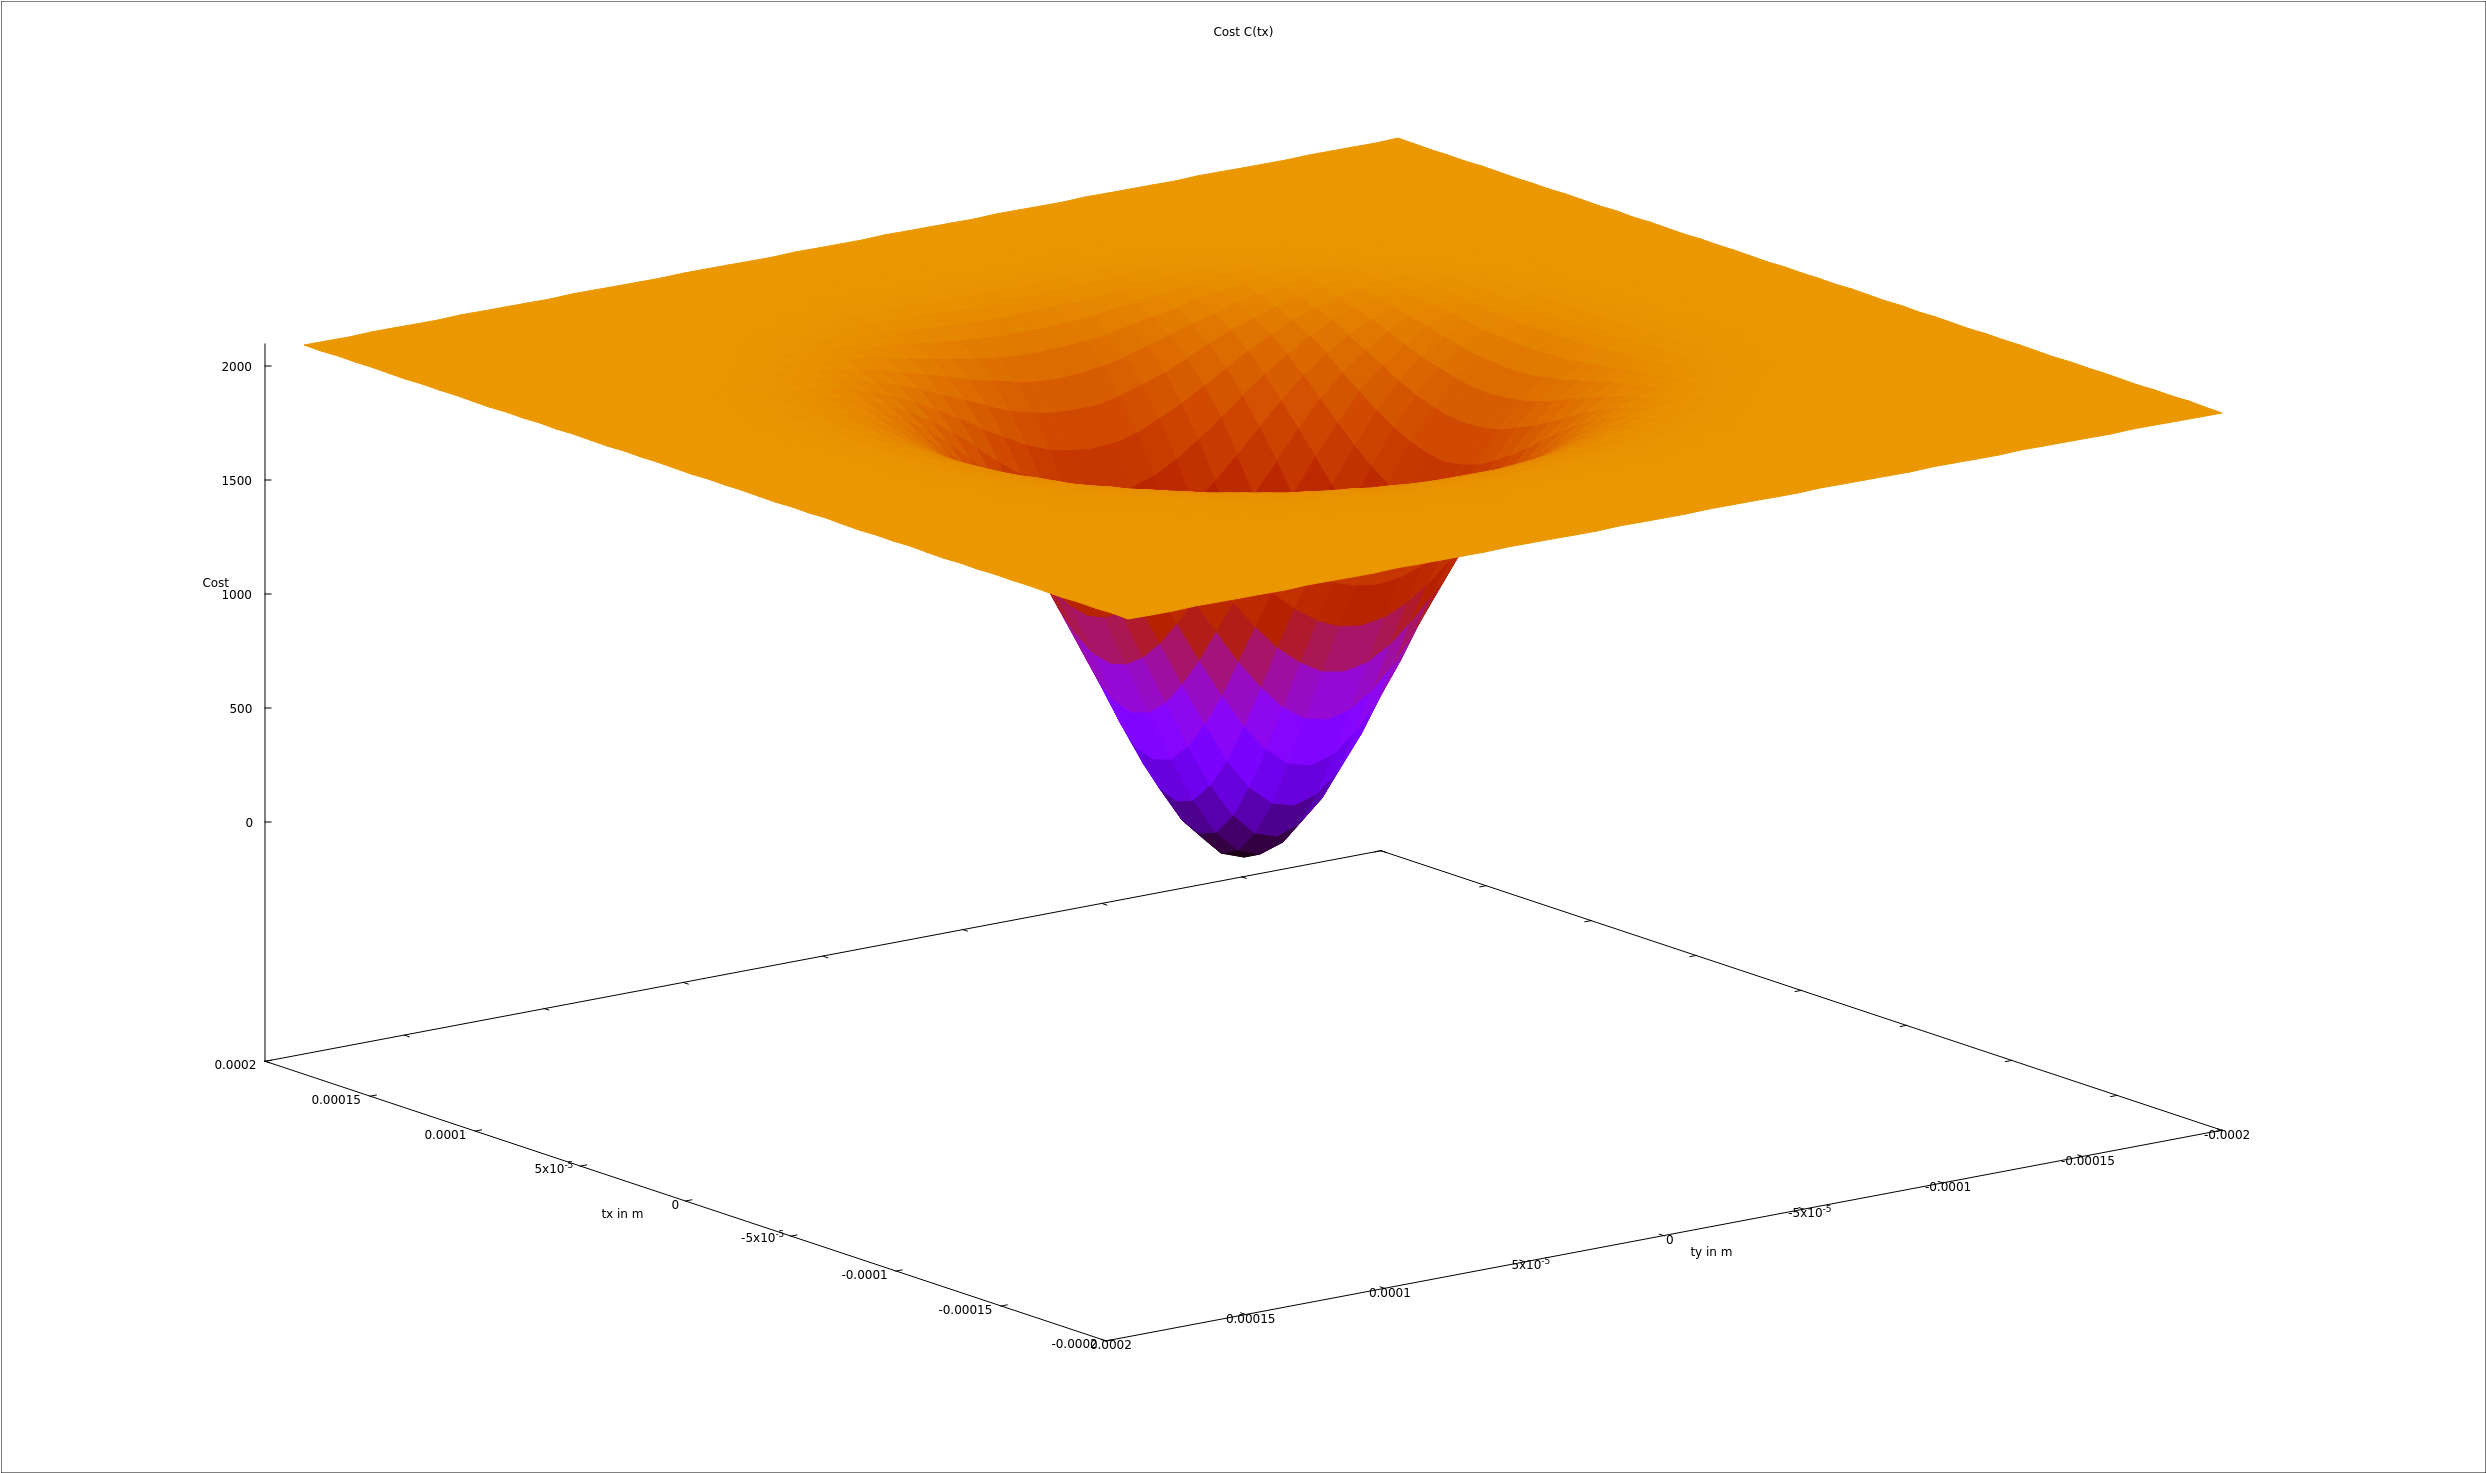
\includegraphics[scale = 0.15]{figures/C(tx,ty).png}
    \caption{Cost function for tx and ty}
    \label{cost_fig}
\end{figure}

 \par We start by expressing the gradient of the cost by applying \eqref{grad_eq}.
 \begin{equation}
    \nabla \textbf{C}(\textbf{t}) = \begin{bmatrix}
        \frac{\partial C}{\partial tx}(\textbf{t})\\
        \frac{\partial C}{\partial ty}(\textbf{t})
    \end{bmatrix}
    \label{grad_eq}
 \end{equation}
 We obtain \eqref{grad_expression}.
 \begin{equation}
    \nabla \textbf{C}(\textbf{t}) = 
    \begin{cases}
        \begin{bmatrix}
            0 \\ 0 
        \end{bmatrix} & \text{if  } tx^{2}+ty^{2} \geq -\frac{(K_{u}Z^{*})^{2}}{f^{2}}8\lambda^2\ln\left(\frac{2\pi\lambda^{2}l}{I_{1}}\right)\\
        \begin{bmatrix}
            \frac{I_{1}^{2}}{4\pi\lambda^{2}}\left(\frac{f^{2}tx}{2(K_{u}Z^{*})^{2}\lambda^{2}}\right)e^{-\frac{f^{2}\left(tx^{2}+ty^{2}\right)}{(2K_{u}Z^{*}\lambda)^{2}}}\\ \frac{I_{1}^{2}}{4\pi\lambda^{2}}\left(\frac{f^{2}ty}{2(K_{u}Z^{*})^{2}\lambda^{2}}\right)e^{-\frac{f^{2}\left(tx^{2}+ty^{2}\right)}{(2K_{u}Z^{*}\lambda)^{2}}} 
        \end{bmatrix} & \text{Otherwise}
    \end{cases} 
    \label{grad_expression}
 \end{equation}
Solving $\nabla \textbf{C}(\textbf{t})= \textbf{0}$, we have two solutions
\begin{itemize}
    \item (tx,ty) = (0,0) which corresponds to the global minimum
    \item $tx^{2}+ty^{2} \geq -\frac{(K_{u}Z^{*})^{2}}{f^{2}}8\lambda^2\ln\left(\frac{2\pi\lambda^{2}l}{I_{1}}\right)$
\end{itemize}
Hence, the region of convergence is then given by \eqref{final_roc1}
\begin{equation}
    \boxed{
        tx^{2}+ty^{2} \geq -\frac{(K_{u}Z^{*})^{2}}{f^{2}}8\lambda^2\ln\left(\frac{2\pi\lambda^{2}l}{I_{1}}\right)
    }
    \label{final_roc1}
\end{equation}
Replacing $\lambda $ by  \eqref{lambda}, the region of convergence is then given by \eqref{final roc}
\begin{equation}
    \boxed{
        tx^{2}+ty^{2} \leq -2\frac{D^{2}(Z^{*}-Z_{f})^{2}}{9(Z_{f}-f)^{2}}ln\left(\frac{2\pi\lambda^{2}l}{I_{1}}\right)
    }
    \label{final roc}
\end{equation}
\bibliographystyle{ieeetr}
\bibliography{biblio.bib}
\end{document}